\documentclass{article}
\usepackage{graphicx, listings, xcolor, subcaption, hyperref}
\usepackage[letterpaper,top=1cm,bottom=2cm,left=1cm,right=1cm,marginparwidth=1cm]{geometry}

\lstset{
  basicstyle=\ttfamily\footnotesize,
  keywordstyle=\color{blue},
  stringstyle=\color{red},
  commentstyle=\color{gray},
  breaklines=true,
  showstringspaces=false,
  backgroundcolor=\color{gray!10}
}

\title{CISC866 Lab Report}
\author{Like Wang}

\begin{document}

\maketitle

\section{Encryption Mode: ECB vs. CBC}

\subsection{Display both encrypted image files}

\textit{Note: I chose to use the following method to get rid of the header issue:}
\begin{lstlisting}[language=Python]
$ head -c 54 original1.bmp > header
$ tail -c +55 encrypted1.bmp > body
$ cat header body > new1.bmp
\end{lstlisting}
\textbf{Encryption command for ECB mode} (Note: iv not used by this cipher):
\begin{lstlisting}[language=Python]
$ openssl enc -aes-128-ecb -e -in pic_original1.bmp -out pic_1_ecb_enc.bmp -K 00112233445566778889aabbccddeeff
$ openssl enc -aes-128-ecb -e -in pic_original2.bmp -out pic_2_ecb_enc.bmp -K 00112233445566778889aabbccddeeff
\end{lstlisting}
Picture look like this:
\begin{figure}[h]
    \centering
    \begin{subfigure}{0.45\textwidth}
        \centering
        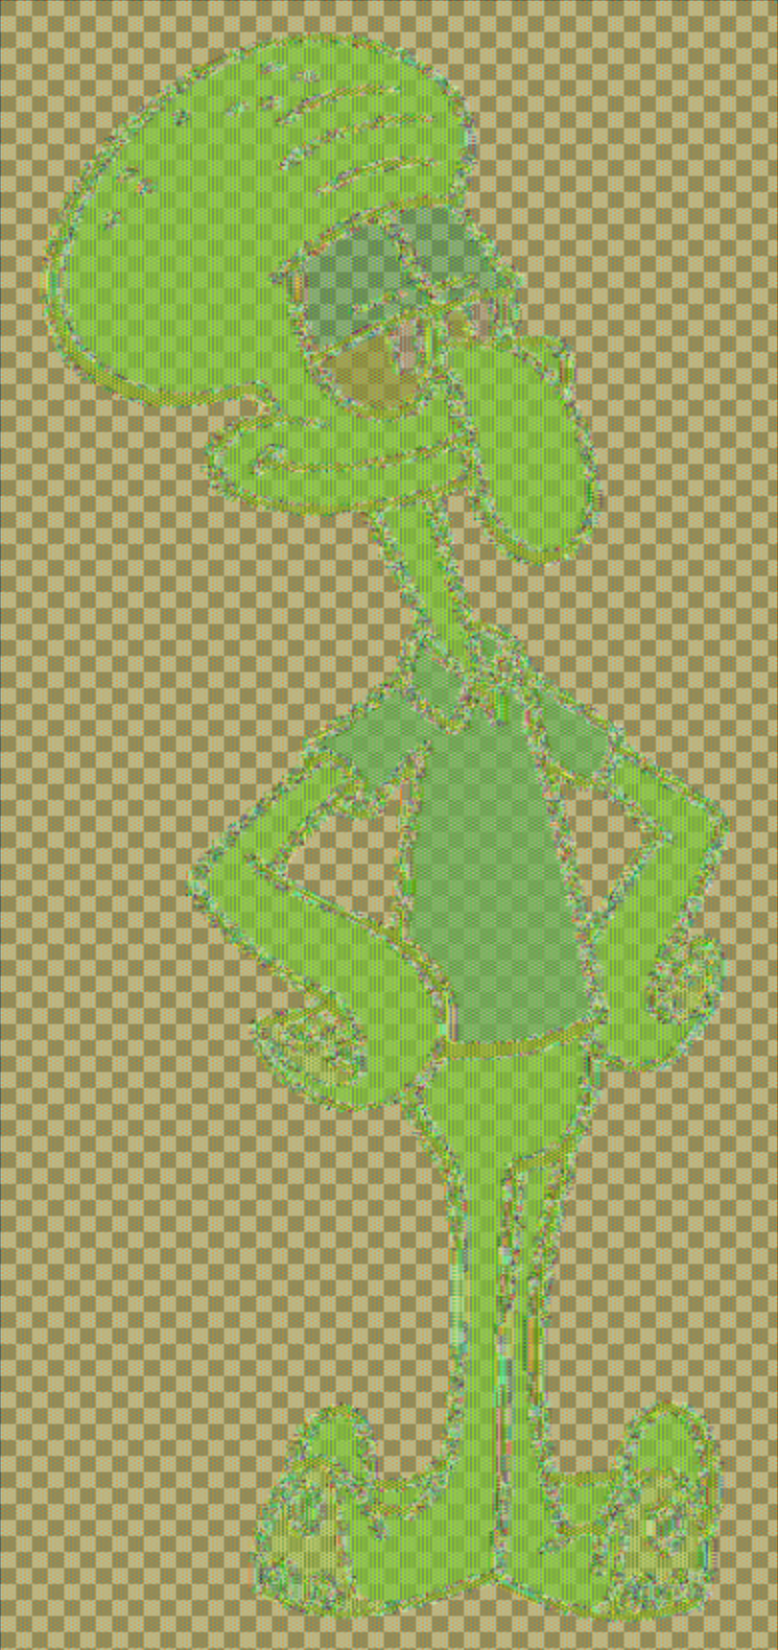
\includegraphics[height=3cm]{images/pic_1_ecb.png}
        \caption{Encrypted pic original1.bmp}
    \end{subfigure}
    \begin{subfigure}{0.45\textwidth}
        \centering
        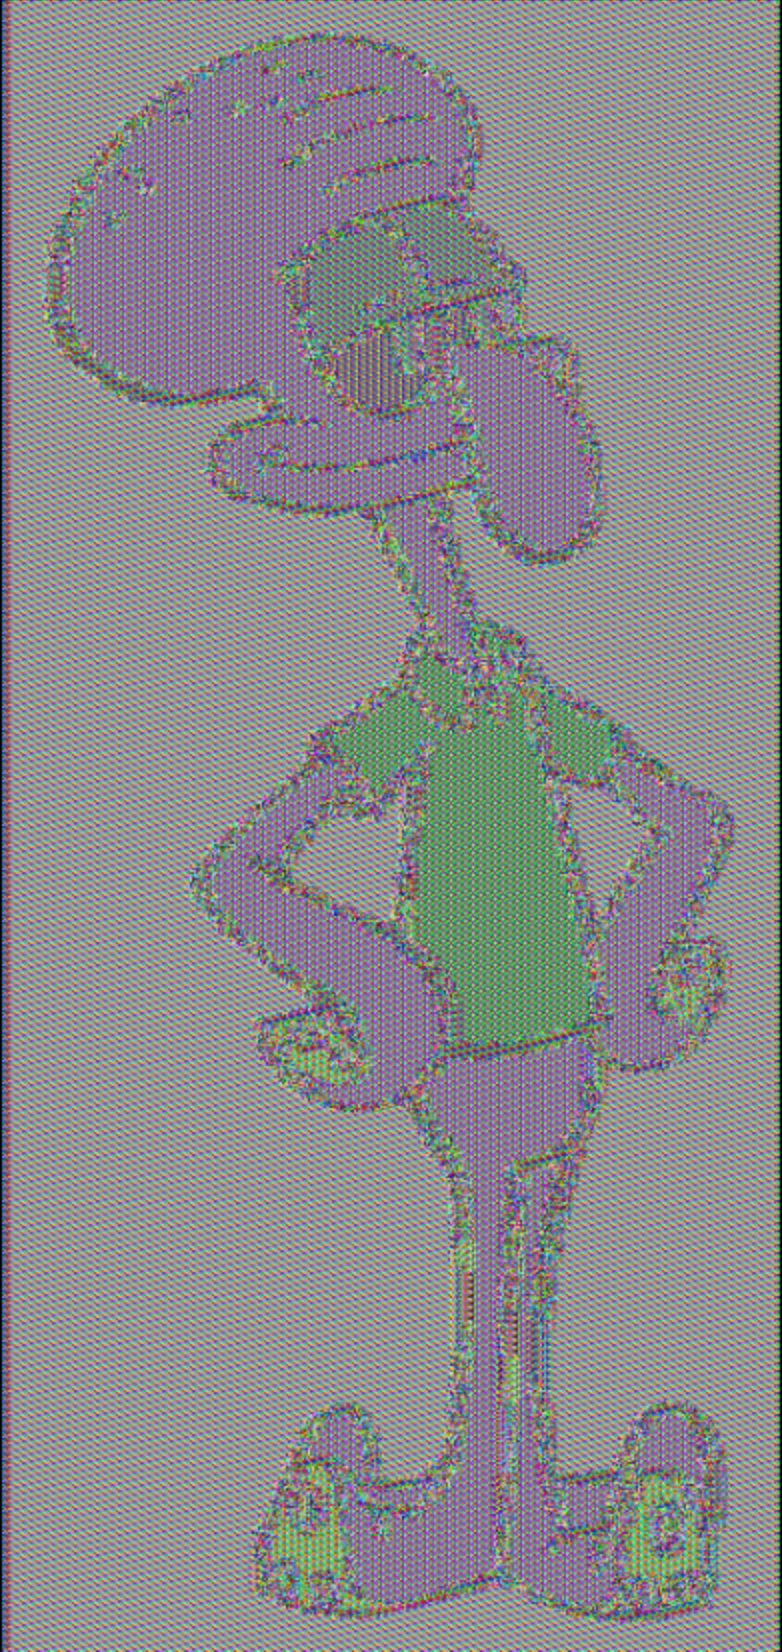
\includegraphics[height=3cm]{images/pic_2_ecb.png}
        \caption{Encrypted pic original2.bmp}
    \end{subfigure}
    \caption{ECB Mode Encrypted Images}
\end{figure}
\textbf{Encryption command for CBC mode}:
\begin{lstlisting}[language=Python]
$ openssl enc -aes-128-cbc -e -in pic_original1.bmp -out pic_1_cbc_enc.bmp -K 00112233445566778889aabbccddeeff -iv 0102030405060708090a0b0c0d0e0f10
$ openssl enc -aes-128-cbc -e -in pic_original2.bmp -out pic_2_cbc_enc.bmp -K 00112233445566778889aabbccddeeff -iv 0102030405060708090a0b0c0d0e0f10
\end{lstlisting}
Picture look like this:
\begin{figure}[h]
    \centering
    \begin{subfigure}{0.45\textwidth}
        \centering
        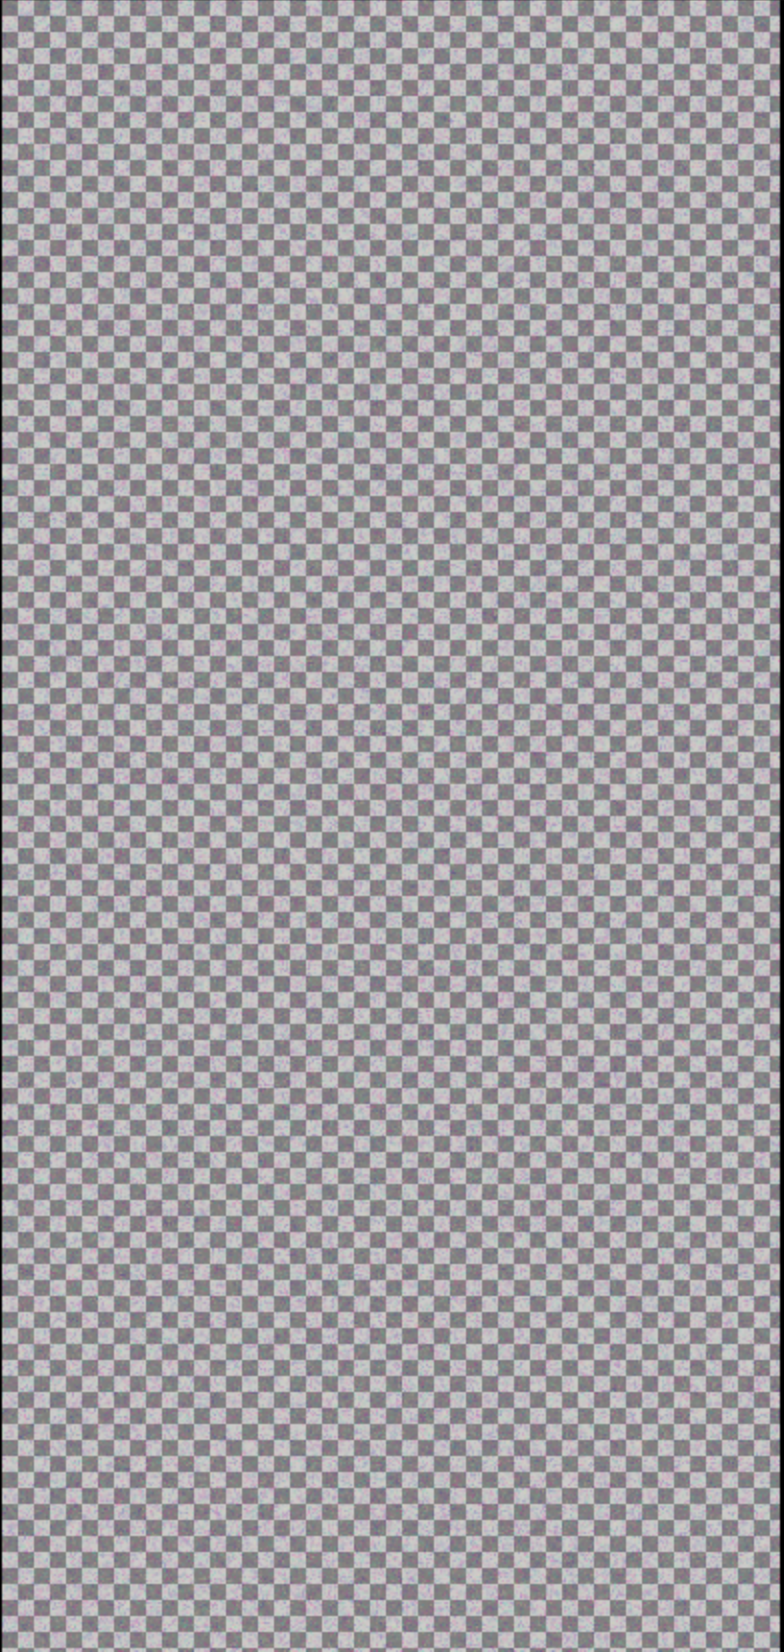
\includegraphics[height=3cm]{images/pic_1_cbc.png}
        \caption{Encrypted pic original1.bmp}
    \end{subfigure}
    \begin{subfigure}{0.45\textwidth}
        \centering
        
\includegraphics[height=3cm]{images/pic_2_cbc.png}
        \caption{Encrypted pic original2.bmp}
    \end{subfigure}
    \caption{CBC Mode Encrypted Images}
\end{figure}
\subsection{Explain my observations}
\begin{itemize}
  \item \textbf{ECB mode} is kind of like a invalid encryption for images, because it reveals patterns in the original image. Even though the colors are changed, the shapes and outlines of objects in the image are still visible.
  \item \textbf{CBC mode} is a much better encryption method, at least from the encrypted cbc images, I can't really tell what the original image looks like.
\end{itemize}
Digging on the reason why, I found that: ECB is weak encryption for images because it's encrypted block wise, meaning that identical plaintext blocks are encrypted into identical ciphertext blocks, while CBC mode uses an initialization vector (IV) and chains the encryption of each block to the previous one, which helps to obscure patterns in the original image.\\
Check the following references for detailed information:\\
\url{https://pycryptodome.readthedocs.io/en/latest/src/cipher/classic.html#ecb-mode}\\
\url{https://pycryptodome.readthedocs.io/en/latest/src/cipher/classic.html#cbc-mode}\\
\url{https://www.highgo.ca/2019/08/08/the-difference-in-five-modes-in-the-aes-encryption-algorithm/}

\subsection{Describe the visual differences}
The original image looks very simmilar, but to me, I first noticed that original1.bmp (1.5 MB) has a bigger file size
than original2.bmp (1.1 MB), then, I tried to zoom both picture, and noticed that original1.bmp has a vector background,
meaning that when I zoom in, the background is still clear.\\
Therefore, the color encoding mechanism (for each pixel) of these 2 images might be different. The second image:
original2.bmp might used RGB color encoding, while original1.bmp might used some other color encoding mechanism.
And note that since AES (CBC and ECB) are block ciphers, meaning that they encrypt fixed size blocks of 128 bits,
so, if we are using RGB color encoding, each pixel is represented by 24 bits, so, each block can only contain
5 pixels (5*24=120 bits) and the remaining 8 bits are carried to the next block. After a certain number of blocks,
the reminder bits will accumulate to 24 bits, and form a new pixel. And that's why we see partern like the image
shown below.\\
\begin{figure}[h]
    \centering
    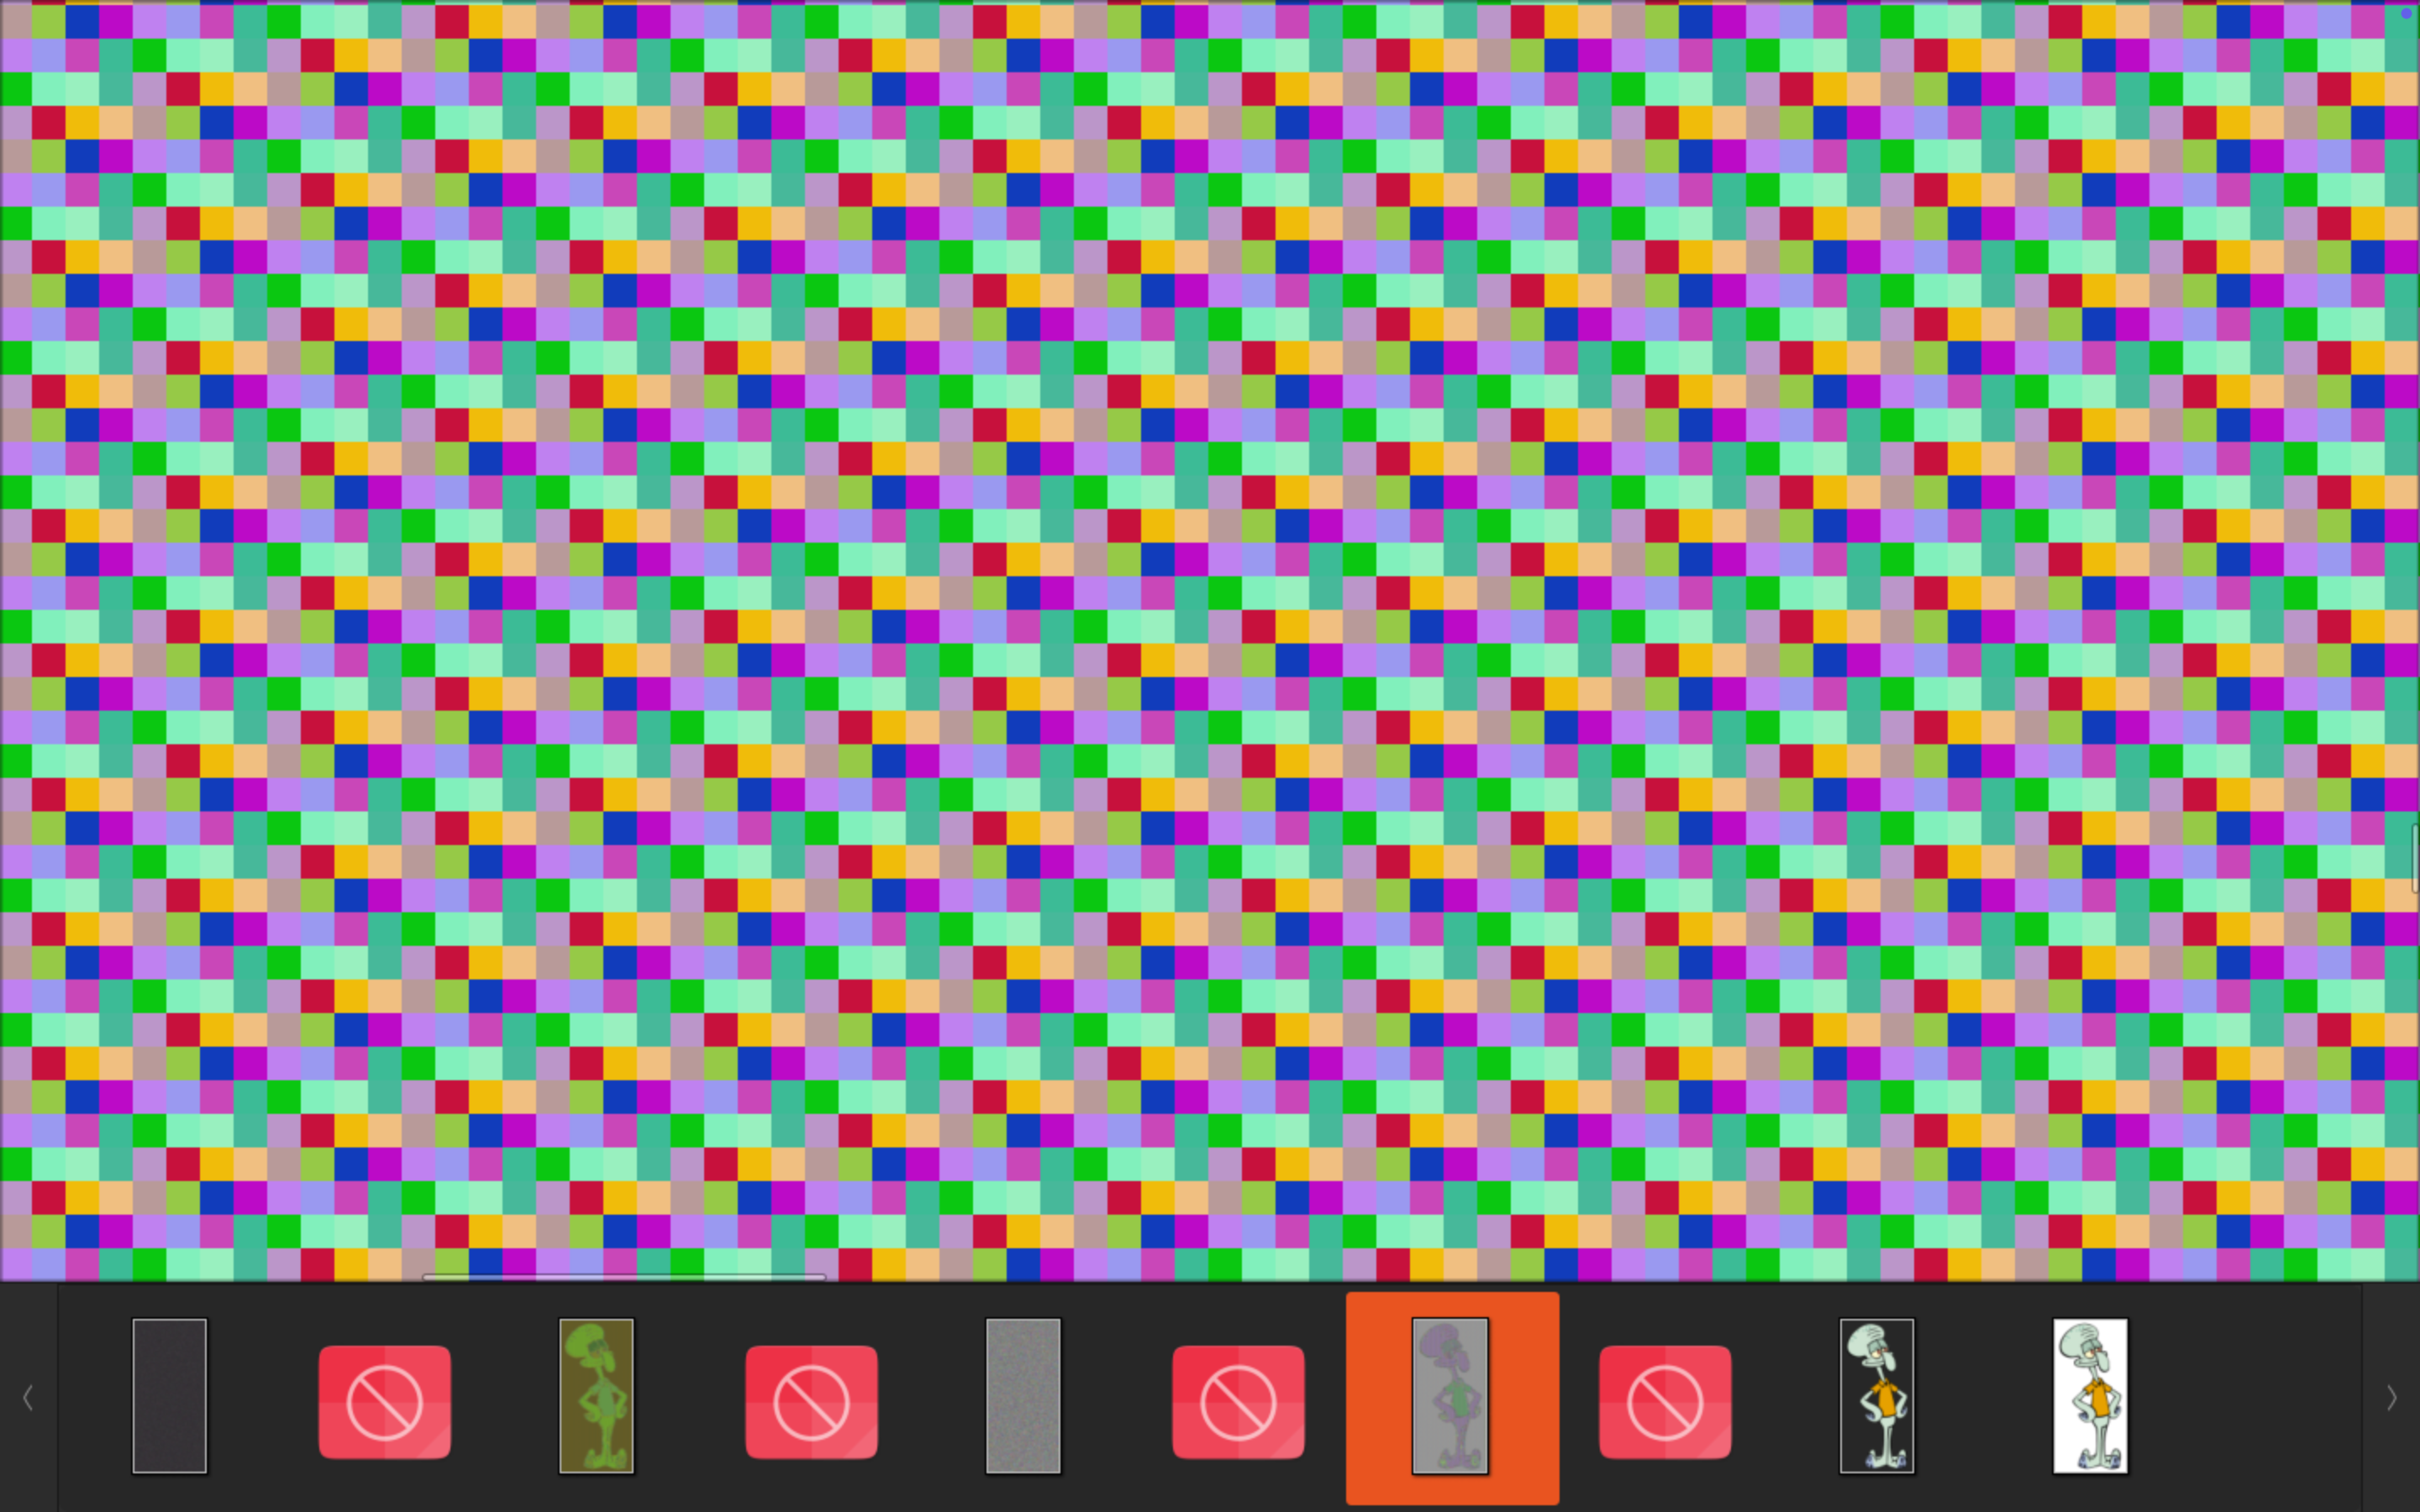
\includegraphics[height=3cm]{images/slash_pattern.png}
    \caption{Zoomed Encrypted pic original2.bmp}
\end{figure}

\section{Padding}
\subsection{Padding for ECB, CBC, CFB, OFB, and CTR modes}
ECB and CBC modes require padding, while CFB, OFB, and CTR modes do not require padding. I was inspired by one the things
Professor mentioned in the lecture: "In CTR modes, we will generate a keystream that is the same length as the plaintext".
I was thinking, that could be the reason why CFB, OFB, and CTR modes do not require padding. I confirmed my guess by
the following references:\\
\url{https://en.wikipedia.org/wiki/Block_cipher_mode_of_operation}\\
\subsection{File Size Comparison after Encrypted with CBC}
I used the following command to create a file:
\begin{lstlisting}[language=Python]
$ echo -n "12345" > f1.txt
$ echo -n "1234567890" > f2.txt
$ echo -n "1234567890asdfga" > f3.txt
\end{lstlisting}
Then I encrypted them using CBC mode:
\begin{lstlisting}[language=Python]
$ openssl enc -aes-128-cbc -e -in f1.txt -out f1_enc.txt -K 00112233445566778889aabbccddeeff -iv 0102030405060708090a0b0c0d0e0f10
$ openssl enc -aes-128-cbc -e -in f2.txt -out f2_enc.txt -K 00112233445566778889aabbccddeeff -iv 0102030405060708090a0b0c0d0e0f10
$ openssl enc -aes-128-cbc -e -in f3.txt -out f3_enc.txt -K 00112233445566778889aabbccddeeff -iv 0102030405060708090a0b0c0d0e0f10
\end{lstlisting}
The file size comparison is shown below:
\begin{table}[h]
\centering
\begin{tabular}{|c|c|c|}
\hline
\textbf{File} & \textbf{Original Size (bytes)} & \textbf{Encrypted Size (bytes)} \\
\hline
f1.txt & 5 & 16 \\
\hline
f2.txt & 10 & 16 \\
\hline
f3.txt & 16 & 32 \\
\hline
\end{tabular}
\caption{File Size Comparison}
\end{table}\\
From the table above, we can see that no matter how many bytes the original file has (as long as it's less than 16 bytes),
the encrypted file size is always 16 bytes. This is because AES is a block cipher that operates on fixed-size blocks of 16 bytes.
When the plaintext is shorter than the block size, padding is added to make it a full block of 16 bytes. However, if the original
file size is exactly 16 bytes, an additional block of padding is added, resulting in an encrypted file size of 32 bytes.
\subsection{Decryption of The CBC Encrypted Files}
I used the following command to decrypt the files:
\begin{lstlisting}[language=Python]
$ openssl enc -aes-128-cbc -d -nopad -in f1_enc.txt -out f1_dec.txt -K 00112233445566778889aabbccddeeff -iv 0102030405060708090a0b0c0d0e0f10
$ openssl enc -aes-128-cbc -d -nopad -in f2_enc.txt -out f2_dec.txt -K 00112233445566778889aabbccddeeff -iv 0102030405060708090a0b0c0d0e0f10
$ openssl enc -aes-128-cbc -d -nopad -in f3_enc.txt -out f3_dec.txt -K 00112233445566778889aabbccddeeff -iv 0102030405060708090a0b0c0d0e0f10
\end{lstlisting}
Let's run \texttt{hexdump} on the decrypted file:
\begin{lstlisting}[language=Python]
$ hexdump -C f1_dec.txt
00000000  31 32 33 34 35 0b 0b 0b  0b 0b 0b 0b 0b 0b 0b 0b  |12345...........|
00000010
$ hexdump -C f2_dec.txt
00000000  31 32 33 34 35 36 37 38  39 30 06 06 06 06 06 06  |1234567890......|
00000010
$ hexdump -C f3_dec.txt
00000000  31 32 33 34 35 36 37 38  39 30 61 73 64 66 67 61  |1234567890asdfga|
00000010  10 10 10 10 10 10 10 10  10 10 10 10 10 10 10 10  |................|
00000020
\end{lstlisting}
We can see that the decrypted files contain padding bytes (\texttt{0x0b, 0x06, 0x10}) at the end of the original data.
\texttt{0x0b} means there are 11 bytes of padding, \texttt{0x06} means there are 6 bytes of padding,
and \texttt{0x10} means there are 16 bytes of padding.

\subsection{Experiments with 256-bit AES}
Let's first try a file with size of 7 and 16 bytes:
\begin{lstlisting}[language=Python]
$ echo -n "1234567" > aes_256_1.txt
$ openssl enc -aes-256-cbc -e -in aes_256_1.txt -out aes_256_1_enc.txt -K 00112233445566778889aabbccddeeff00112233445566778889aabbccddeeff -iv 0102030405060708090a0b0c0d0e0f10
$ openssl enc -aes-256-cbc -d -nopad -in aes_256_1_enc.txt -out aes_256_1_dec.txt -K 00112233445566778889aabbccddeeff00112233445566778889aabbccddeeff -iv 0102030405060708090a0b0c0d0e0f10
$ hexdump -C aes_256_1_dec.txt
00000000  31 32 33 34 35 36 37 09  09 09 09 09 09 09 09 09  |1234567.........|
00000010
$ echo -n "1234567890abcdef" > aes_256_2.txt
$ openssl enc -aes-256-cbc -e -in aes_256_2.txt -out aes_256_2_enc.txt -K 00112233445566778889aabbccddeeff00112233445566778889aabbccddeeff -iv 0102030405060708090a0b0c0d0e0f10
$ openssl enc -aes-256-cbc -d -nopad -in aes_256_2_enc.txt -out aes_256_2_dec.txt -K 00112233445566778889aabbccddeeff00112233445566778889aabbccddeeff -iv 0102030405060708090a0b0c0d0e0f10
$ hexdump -C aes_256_2_dec.txt
00000000  31 32 33 34 35 36 37 38  39 30 61 62 63 64 65 66  |1234567890abcdef|
00000010  10 10 10 10 10 10 10 10  10 10 10 10 10 10 10 10  |................|
00000020
\end{lstlisting}
The original file size is 16 bytes, the encrypted file size is 32 bytes (which is expected)\\
Now let's try a file with size of 47 bytes:
\begin{lstlisting}[language=Python]
$ echo -n "This is a test file for 256-bit AES encryption." > aes_256_3.txt
$ openssl enc -aes-256-cbc -e -in aes_256_3.txt -out aes_256_3_enc.txt -K 00112233445566778889aabbccddeeff00112233445566778889aabbccddeeff -iv 0102030405060708090a0b0c0d0e0f10
$ openssl enc -aes-256-cbc -d -nopad -in aes_256_3_enc.txt -out aes_256_3_dec.txt -K 00112233445566778889aabbccddeeff00112233445566778889aabbccddeeff -iv 0102030405060708090a0b0c0d0e0f10
$ hexdump -C aes_256_3_dec.txt
00000000  54 68 69 73 20 69 73 20  61 20 74 65 73 74 20 66  |This is a test f|
00000010  69 6c 65 20 66 6f 72 20  32 35 36 2d 62 69 74 20  |ile for 256-bit |
00000020  41 45 53 20 65 6e 63 72  79 70 74 69 6f 6e 2e 01  |AES encryption..|
00000030
\end{lstlisting}
The original file size is 47 bytes, the encrypted file size is 48 (which is 32+16) bytes, which behaves exactly like 128-bit AES's padding mechanism. \\


\end{document}